\documentclass{article}

\usepackage{tikz}
\usepackage{float}
\usepackage{multirow}
\usepackage[margin=1in]{geometry}

\graphicspath{ {.} }

\title{
    Manutenção Inteligente em Cenário de Indústria 4.0 \\
    \vspace{0.75em}
    \Large Entrega 1 \\  \vspace{1.25em} 
    \large
    \begin{tabular}{rl}
        \textbf{Turno:}& MODL03 \\ 
        \rule{0pt}{1.25em} 
        \textbf{Docente:}& Maria do Rosário Bernardo 
    \end{tabular}
}
\author{}
\date{}


\begin{document}
    \maketitle
    \begin{tikzpicture}[overlay, remember picture]
        \node[xshift=3.5cm,yshift=-2.5cm] at (current page.north west) {
\includegraphics[scale = 0.35]{logo_ist.jpeg}};
    \end{tikzpicture}

    \begin{table}[H]
        \centering
        \begin{tabular}{|l|l|l|l|l}
        \cline{1-4}
        \multicolumn{1}{|l|}{}                   & \multicolumn{1}{l|}{}       & \multicolumn{1}{l|}{}                             & \multicolumn{1}{l|}{}                   &  \\
        \multicolumn{1}{|l|}{}                   & \multicolumn{1}{l|}{}       & \multicolumn{1}{l|}{}                             & \multicolumn{1}{l|}{}                   &  \\
        \multicolumn{1}{|c|}{Nome}               & \multicolumn{1}{c|}{Número} & \multicolumn{1}{c|}{Esforço estimado de trabalho} & \multicolumn{1}{c|}{Tarefas realizadas} &  \\
        \multicolumn{1}{|l|}{}                   & \multicolumn{1}{l|}{}       & \multicolumn{1}{l|}{}                             & \multicolumn{1}{l|}{}                   &  \\
        \multicolumn{1}{|l|}{}                   & \multicolumn{1}{l|}{}       & \multicolumn{1}{l|}{}                             & \multicolumn{1}{l|}{}                   &  \\ \cline{1-4}
        \multicolumn{1}{|l|}{}                   & \multicolumn{1}{l|}{}       & \multicolumn{1}{l|}{}                             & \multirow{10}{7cm}{Todas as tarefas do projeto foram executadas em igual parte por ambos os elementos do grupo, com constante revisão e alteração do trabalho feito.
        Começámos por retirar toda a informação relevante do UoD e fazer uma separação inicial dos elementos pelas três camadas (Business, Application e Technology) e  de seguida desenvolvemos, concomitantemente, o modelo Archi.}                   &   \\
        \multicolumn{1}{|l|}{}                   & \multicolumn{1}{l|}{}       & \multicolumn{1}{l|}{}                             & \multicolumn{1}{l|}{}                   &  \\
        \multicolumn{1}{|c|}{Sebastião Assunção} & \multicolumn{1}{c|}{95536}  & \multicolumn{1}{c|}{10 horas}                     & \multicolumn{1}{l|}{}                   &  \\
        \multicolumn{1}{|l|}{}                   & \multicolumn{1}{l|}{}       & \multicolumn{1}{l|}{}                             & \multicolumn{1}{l|}{}                   &  \\
        \multicolumn{1}{|l|}{}                   & \multicolumn{1}{l|}{}       & \multicolumn{1}{l|}{}                             & \multicolumn{1}{l|}{}                   &  \\ \cline{1-3}
        \multicolumn{1}{|l|}{}                   & \multicolumn{1}{l|}{}       & \multicolumn{1}{l|}{}                             & \multicolumn{1}{l|}{}                   &  \\
        \multicolumn{1}{|l|}{}                   & \multicolumn{1}{l|}{}       & \multicolumn{1}{l|}{}                             & \multicolumn{1}{l|}{}                   &  \\
        \multicolumn{1}{|c|}{Duarte Almeida}     & \multicolumn{1}{c|}{95565}  & \multicolumn{1}{c|}{10 horas}                     & \multicolumn{1}{l|}{}                   &  \\
        \multicolumn{1}{|l|}{}                   & \multicolumn{1}{l|}{}       & \multicolumn{1}{l|}{}                             & \multicolumn{1}{l|}{}                   &  \\
        \multicolumn{1}{|l|}{}                   & \multicolumn{1}{l|}{}       & \multicolumn{1}{l|}{}                             & \multicolumn{1}{l|}{}                   &  \\ \cline{1-4}
        \end{tabular}
        \end{table}

    \pagebreak

    \vspace*{3cm}

    \begin{figure}[H]
        \centering
        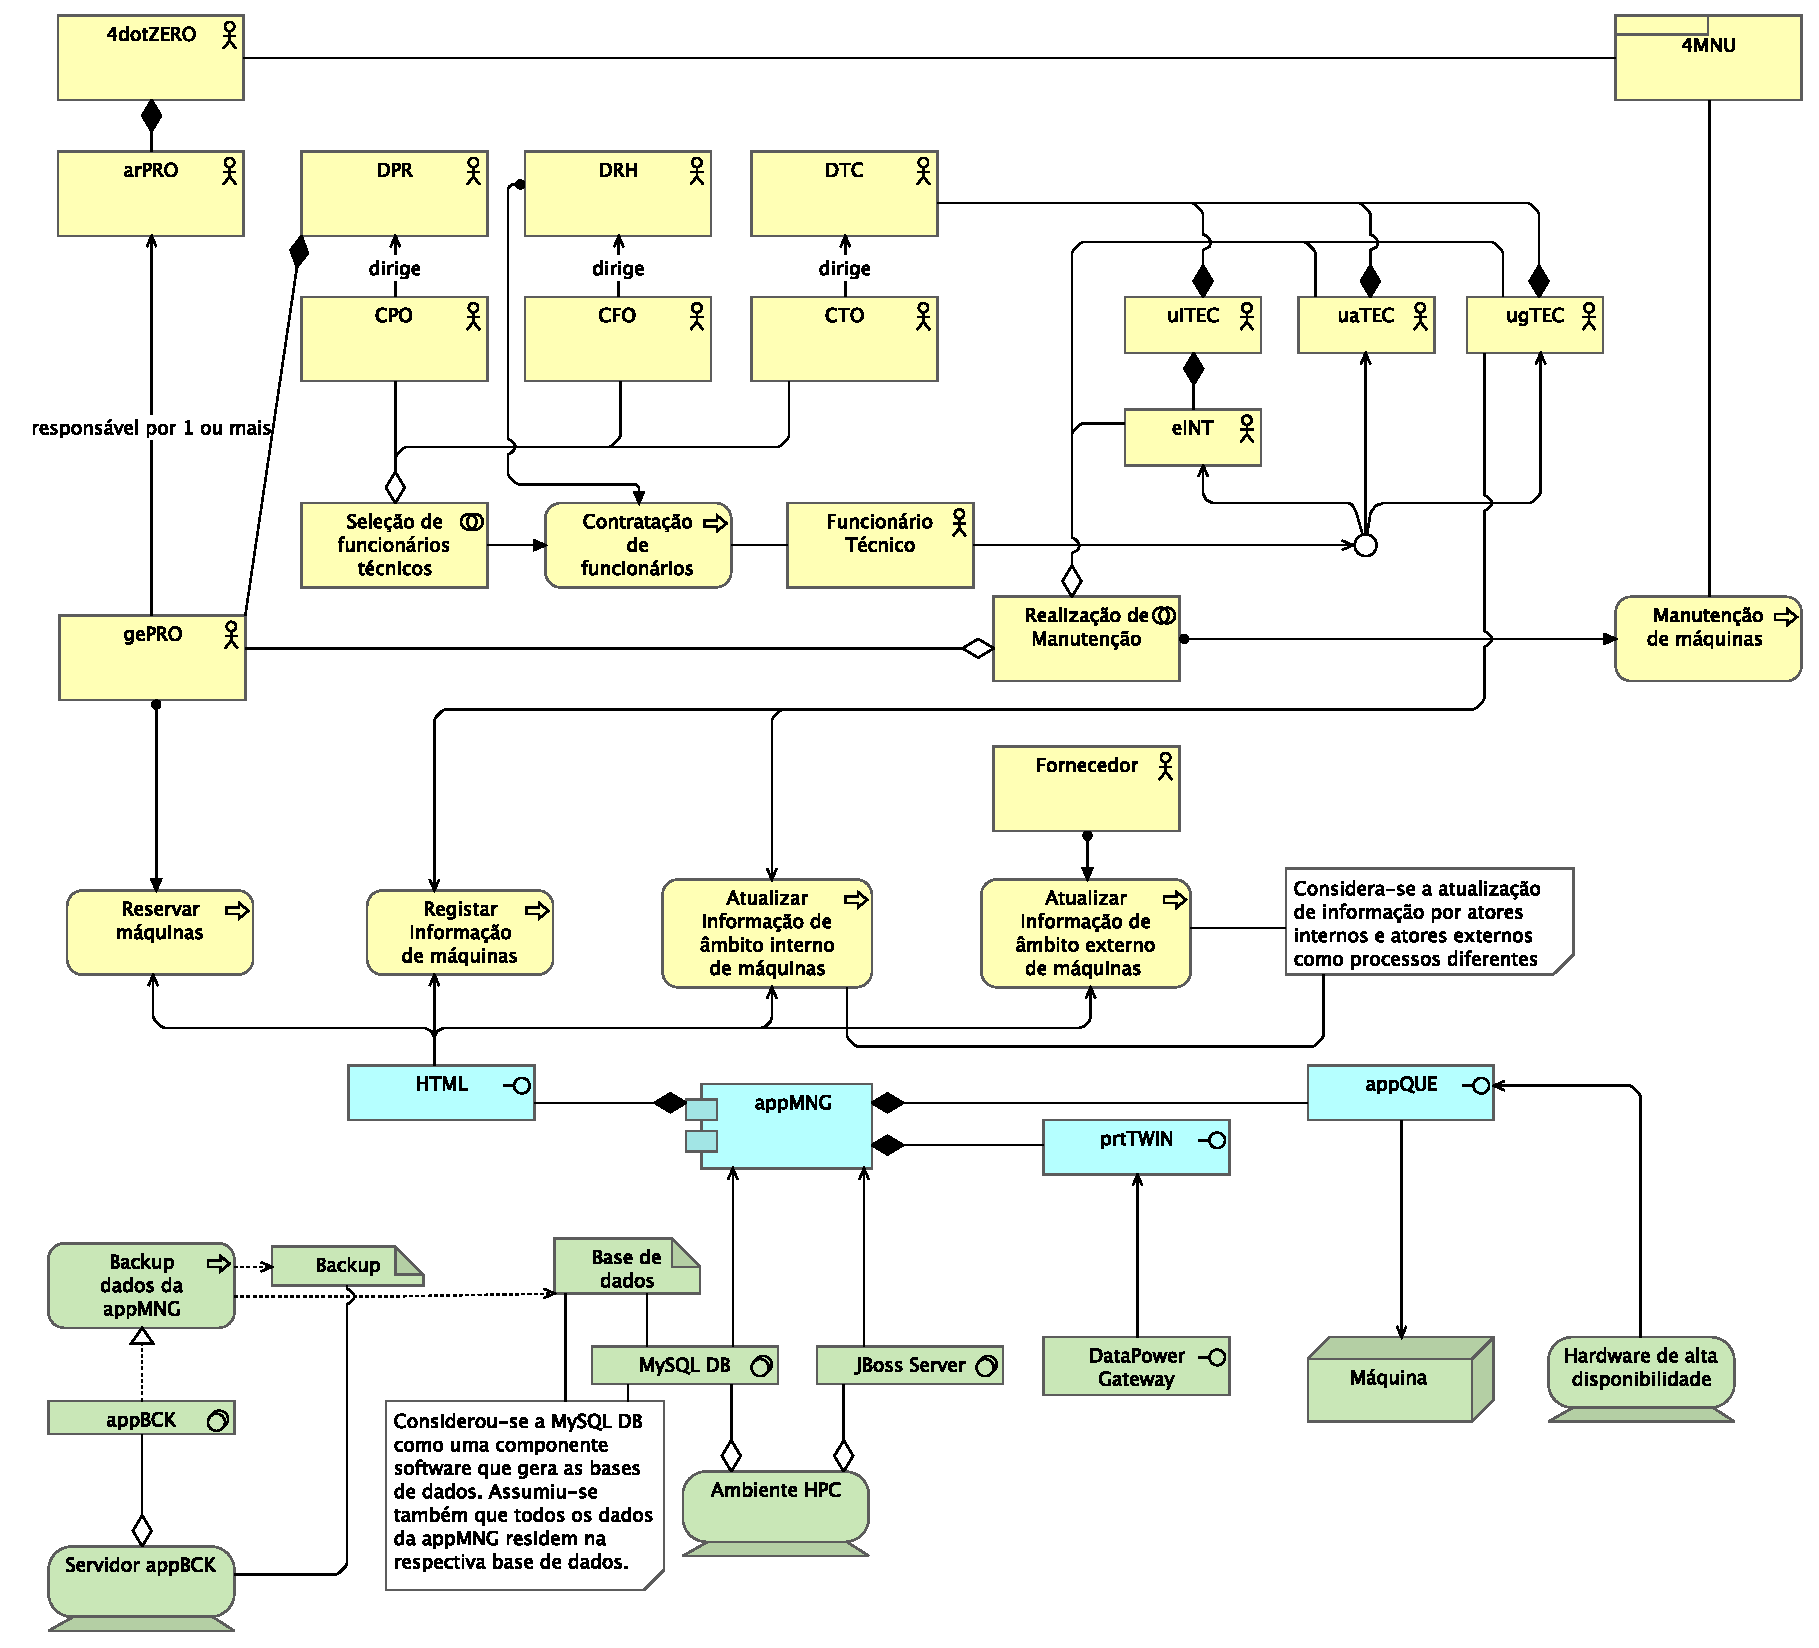
\includegraphics[width=\textwidth]{modelo.pdf}
    \end{figure}

\end{document}